\section{Neighbouring Nodes}\label{sec:neighboring_nodes}
This section starts with a conceptual overview of how neighbouring nodes in an ontology graph are used to generate contextual information. Then, existing approaches on generating textual definitions are examined. In the literature~\cite{soton265735} this task is also known under the term \textit{ontology verbalisation}. Even though there exists \textit{OWL Verbalizer}\footnote{\url{http://mcs.open.ac.uk/nlg/SWAT/Verbaliser.html} accessed 2018/04/30}, a tool which already transforms generic ontologies into English sentences, we could not integrate it into the context enrichment process because 
\begin{inparaenum}[a)]
		\item it was designed as a standalone tool written in SWI-Prolog\footnote{\url{http://www.swi-prolog.org/} accessed 2018/04/30} and
		\item it only accepts the whole ontology as input
\end{inparaenum}.
However, in our approach we adopted some of the rules proposed by OWL~Verbalizer and integrated them in the enrichment process.

To illustrate the concept of neighbouring nodes and how they relate to the context enrichment approach explained later, a simple ontology graph describing the teacher/pupil domain is given in~\hyperref[fig:simple_owl_graph]{Figure~\ref*{fig:simple_owl_graph}}.
\begin{figure}
	 \centering
	 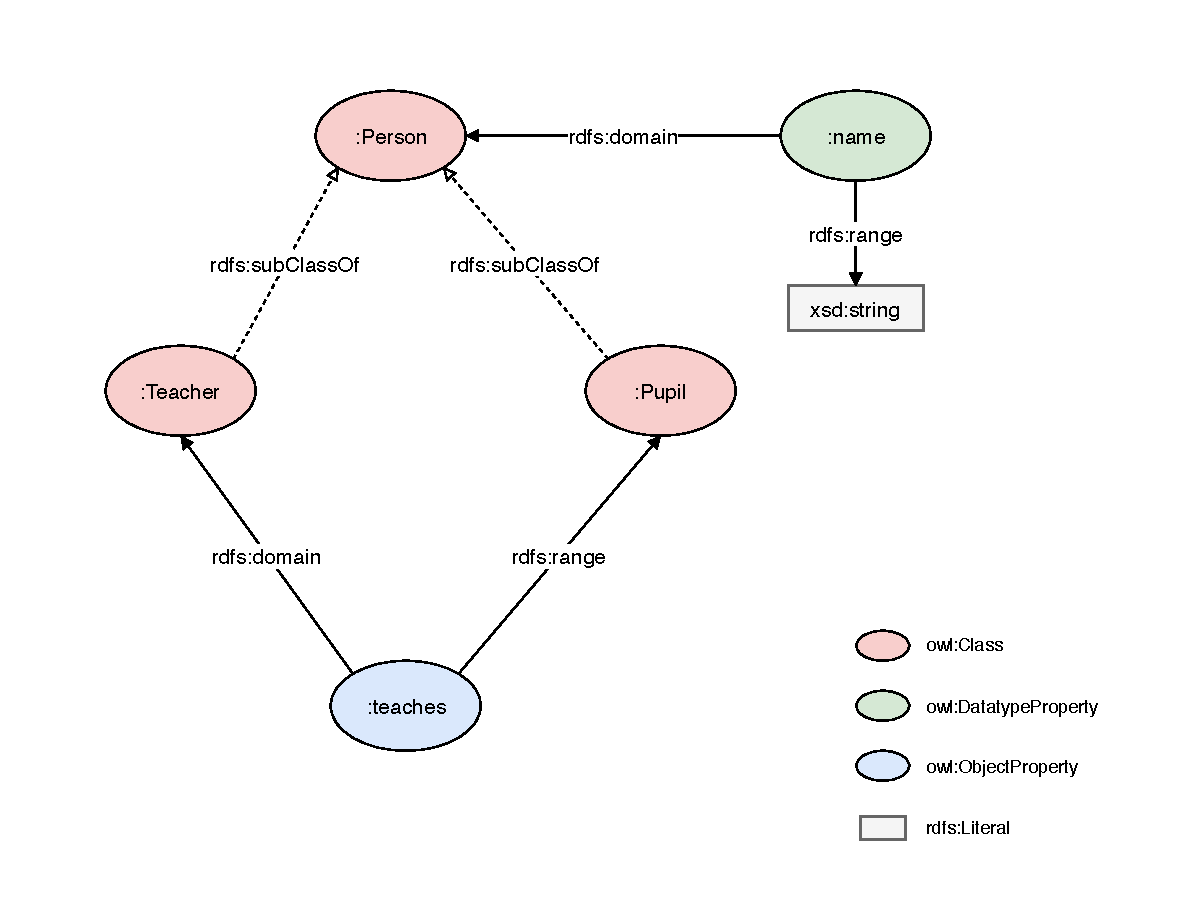
\includegraphics[width=\textwidth]{drawio/University_Ontology_Example}
	 \caption{Simple Ontology Graph}\label{fig:simple_owl_graph}
\end{figure}
For example, if the concept \textit{:Teacher} is taken as reference node, it makes sense to not only include the concept itself, but to also consider connected nodes~(e.g. the concept \textit{:Person} and the object property \textit{:teaches}) as well. 

As in the guidelines for conducting crowdsourcing research~\cite{sarasua2015crowdsourcing}, the authors recommended to avoid technical terms in crowdsourcing questions. In the next paragraphs we explain how \textit{ontology verbalisation} helps to achieve this goal. 

Despite the fact that natural language is desirable for descriptions as everybody knows and understands with no extra learning effort, it conflicts in terms of expressiveness and specificity with well defined ontologies which can encode complex data and relations in domain-specific areas. To resolve this conflict, a new language variant named \textbf{ACE}~\textit{(Attempto Controlled English)}~\cite{fuchs2008} was created. ACE is a formal language, capable of expressing domain-specific knowledge with a well defined syntax, supporting formal reasoning and readable by specialists who are yet unfamiliar with formal languages and methods.

To get a better understanding of ACE\footnote{\url{https://tinyurl.com/yc3zhu9a} accessed 2018/05/05}\footnote{\url{https://tinyurl.com/ycst39jv} accessed 2018/05/05}, a short overview of its language structure is given in the next paragraphs:
 
\paragraph{Simple Sentences} A Simple Sentence derived from standard English language contains a subject, a verb and additional elements: \texttt{subject + verb + complements~[~+~adjuncts~]}. The verb relates directly or indirectly to one or more other objects~(\textit{complements}). Optionally, to add more specificity, one or more adverbs and prepositional phrases can be added~(\textit{adjuncts}). 

\paragraph{Composite Sentences} A Composite Sentence is composed of one or more Simple~Sentences, connected by \textit{coordination},
\textit{subordination}, \textit{quantification} and \textit{negation}. Whereas coordination links sentences either by the word \texttt{and} or \texttt{or}, subordination relates dependent sentences in some way~(e.g. if-then sentences). Quantification allows statements about all~(universal quantification) or certain~(existential quantification) objects of a certain domain. Last, encoding negative polarity in a sentence~(e.g. sentences containing \texttt{not} or \texttt{no}) is defined as negation. 

\paragraph{Query Sentences} Query Sentences can be divided into polar questions~(e.g. with \textit{yes/no} answer) and non-polar questions, also known as \emph{wh-questions}. In contrast to yes/no questions no pre-defined answer exist for these. Furthermore, wh-questions start with either of the following five W-words: \texttt{Who}, \texttt{What}, \texttt{When}, \texttt{Where} and \texttt{Why}. However, this definition somewhat less strict as sometimes questions starting with the word \texttt{How} are included as well.

\paragraph{Anaphoric References} If the meaning of a word or phrase is context dependent, recurring occurrences of these expressions are called \textit{Anaphoric References}. More specifically, the referring term~(\textit{anaphor}) relates to an antecedent expression. For example, given the sentence: \texttt{Tom arrived, but nobody noticed him}, the pronoun \texttt{him} relates to \texttt{Tom}. To resolve ambiguities during the processing phase, Anaphoric References are replaced by encoded references. 

\textbf{OWL Verbalizer}~\cite{stevens2011}, an open source tool aimed at producing texts from generic OWL ontologies, is a good example of a successful integration of ACE. A description of the basic concepts of OWL Verbaliser is given below:

This tool, being now part of the \textbf{SWAT Tool Suite}\footnote{\url{http://mcs.open.ac.uk/nlg/SWAT/} accessed 2018/05/06}, was created to overcome the burden of maintaining ontology definitions by hand. Whereas producing high quality texts in restricted application domains is under active research, this tool produces understandable descriptions using general-purpose methods that are of moderate quality.

The high-level process of ontology verbalisation shown in \hyperref[fig:verbaliser_architecture]{Figure~\ref*{fig:verbaliser_architecture}} consists of the following stages:

\paragraph{Transcoding from OWL to Prolog} The output of this stage is a file in a convenient Prolog format which was generated from an ontology in RDF/XML format. The conversation process covered by the \textit{Transcoder}, \textit{Identifier~Selector} and \textit{Label~Selector} combines identifiers~(concepts, individuals, object~properties) and labels. In addition, ambiguous terms in identifiers are normalised. 

\paragraph{Constructing a lexicon for atomic entities} The output of this stage, covered by the component \textit{Lexicon Generator}, is a collection of lexicons, computed from the normalised Prolog terms in the previous stage. A lexical entry~(lexicon) is defined as a quadruple having the following form: \texttt{<identifier, part-of-speech, singular-form, plural-form>} To facilitate processing in later stages, normalised identifiers for concepts, individuals and object~properties are stored together with word category, singular form and plural form. The word~category, also known as part-of-speech, groups words based on similar properties in terms of syntax and grammar. Common categories are nouns, verbs and adjectives. Last, to differentiate the quantity of a phrase or word, singular and plural form of a noun are associated with each lexical entry. 
Among the storage of lexicons, the algorithm also implements other rules regarding text processing. Some simple heuristics are used for pre-processing to transform the resulting word string into better readable English sentences. 

\paragraph{Selecting the axioms relevant for describing each class} This stage and the next stage are covered by the \textit{Planner}.
This component has as input all axioms from the source ontology as well as the lexicons from the previous stage. In this stage, axioms are mapped to matching lexical entries. As matching criteria the algorithm uses the lexicon identifier and the IRI~\cite{rfc3987}. 

\paragraph{Aggregating axioms with a similar structure} This stage is optional, as it is not strictly required for text generation which is described in the next stage. However, some improvements are achieved if similar axioms are aligned. 

\paragraph{Generating sentences from axioms} The final stage is covered by the component named \textit{Realiser} which forms the central part of the
verbalisation process. English sentences are generated for each axiom using logical rules for almost every logical pattern in OWL-DL. These rules are expressed in Prolog clauses, taking the axiom and optionally the lexicon as input.

\begin{figure}
	 \centering
	 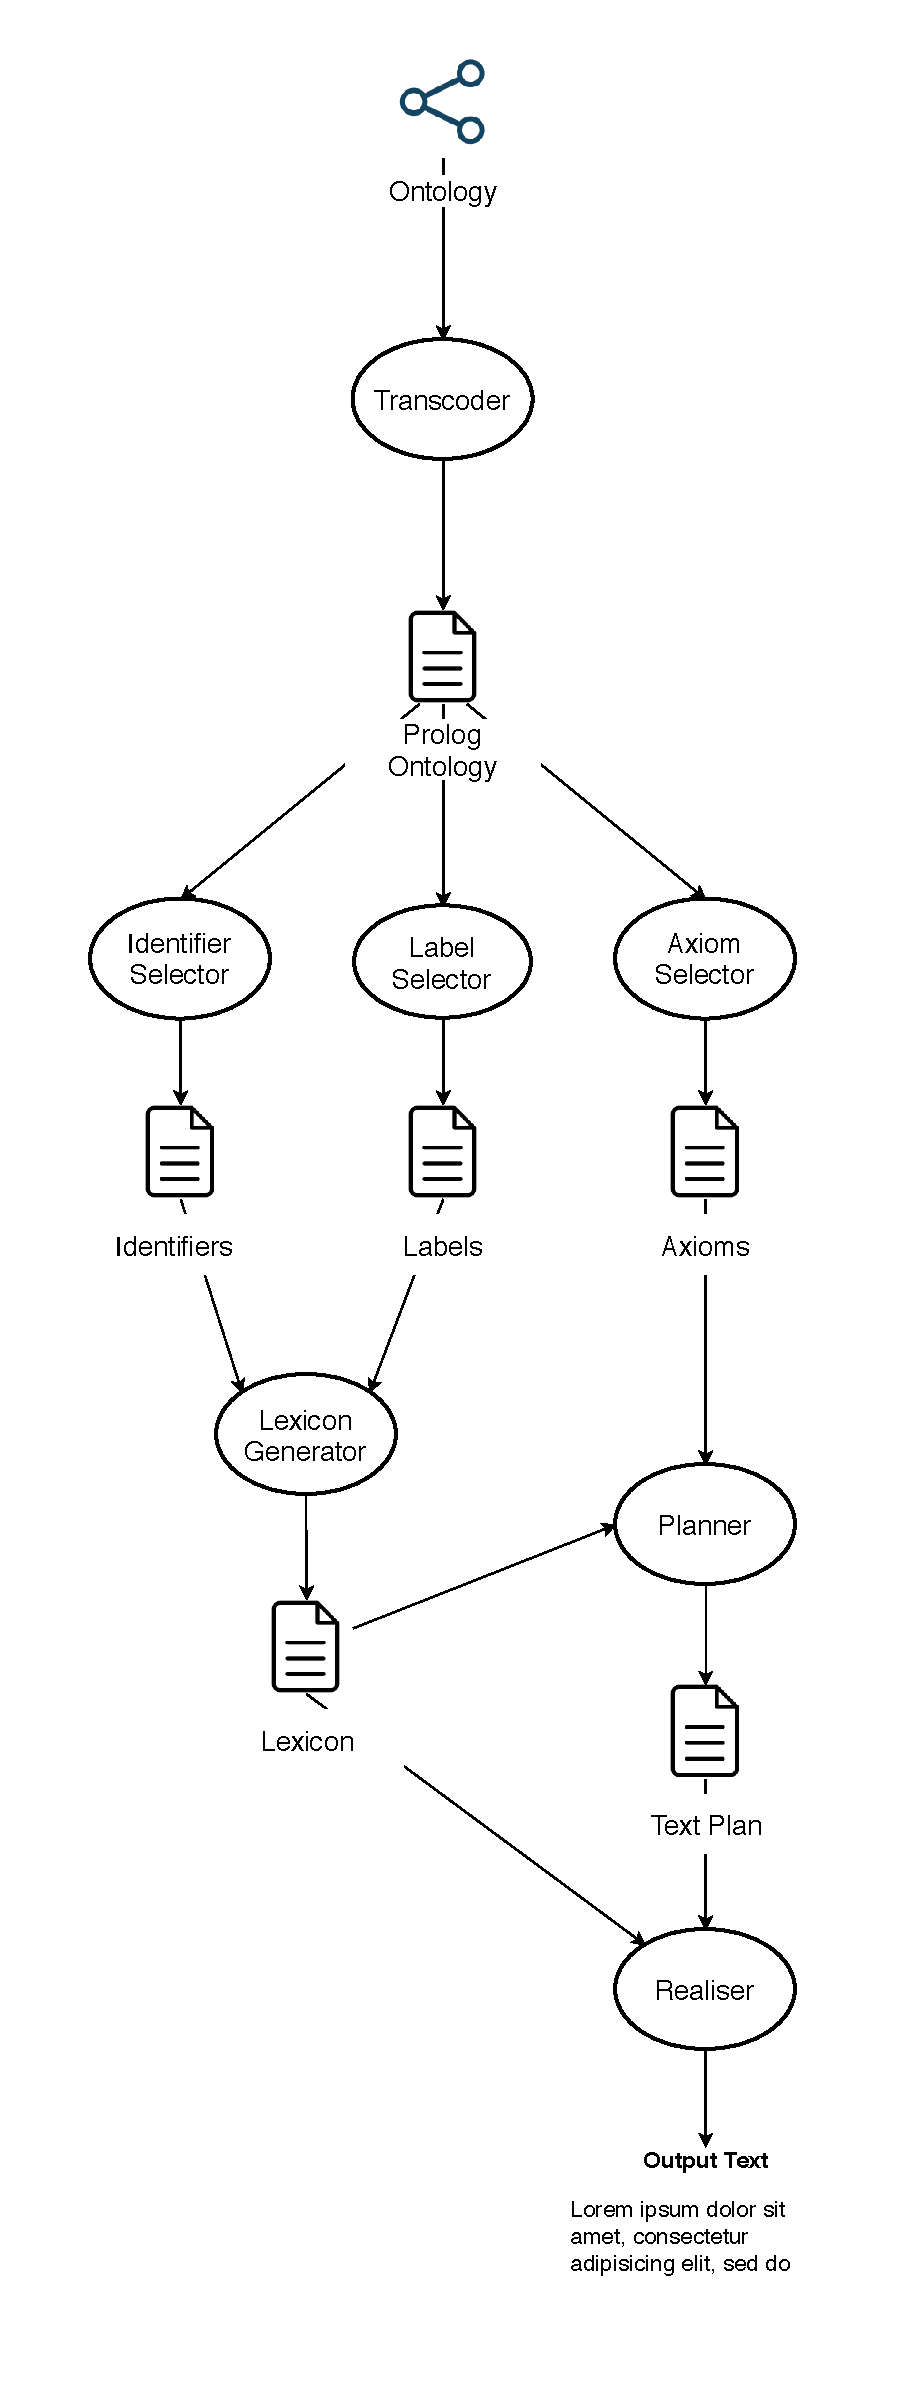
\includegraphics[width=0.5\textwidth]{drawio/Ontology_Verbaliser_Architecture}
	 \caption{Conceptual architecture of the OWL ontology verbaliser~\cite{stevens2011}}\label{fig:verbaliser_architecture}
\end{figure}

Although OWL~Verbaliser would be useful to integrate in the enrichment process, there are some major obstacles:

The first is \textbf{incompatibility on a language level}. Traditionally, software systems are written in many different programming languages, leading to the challenge of dealing with interoperability~\cite{malone2014}. While OWL~Verbaliser was written in SWI-Prolog, Protege runs on the Java Virtual Machine~(JVM), causing a conceptual mismatch in programming languages and paradigms. Moreover, interoperability between conceptually different programming languages is challenging in its own\footnote{\url{http://www.swi-prolog.org/packages/jpl/} accessed 2018/05/11} and would conflict with the goal of an easy-to-integrate solution.

Another obstacle is a \textbf{mismatch on the scope of operation}. OWL~Verbaliser was implemented as a tool assisting engineers in ontology creation, a very time consuming task. It was designed as a standalone tool, launched from the command line or deployed as a web service. On the other hand, ontology enrichment is embedded in Protege and part of the ontology validation process, operating only on small parts of the ontology. In contrast, OWL~Verbaliser takes the whole ontology as input. 

\paragraph{Ontology based Approach}\label{sec:enrichment_ontology_approach}
Due to this complicating issues, we implemented a different approach using some insights from OWL~Verbaliser. The pseudocode of the overall workflow is given in \hyperref[alg:neighbourhood]{Algorithm~\ref*{alg:neighbourhood}}. The notation to describe properties and relations is based on a formal Ontology~Description Logic~(DL)~\cite{baader2003}, string manipulations were formally defined in~\cite{hopcroft1969}.

\begin{algorithm}
	\caption{Context Enrichment based on Neighbouring Nodes}\label{alg:neighbourhood}
	\begin{algorithmic}[1]
		\Procedure{Generate Description}{}\newline
			\textbf{Input:} A concept $C$\newline
			\textbf{Output:} A textual description $T$ of $C's$ neighbouring nodes based on subsumption\newline
			\State{$T=\{\}$} \label{alg:neighbourhood:text_initialisation}
			\For {$ (c,d) \in C \sqsubseteq D $}
				\State $T=T$ $\cup$ "Every " $\cup$ $name(c)$ $\cup$ " is a " $\cup$ $name(d)$
			\EndFor
			\For {$ (e,c) \in E \sqsubseteq C $}
				\State $T=T$ $\cup$ "Every " $\cup$ $name(e)$ $\cup$ " is a " $\cup$ $name(c)$
			\EndFor
		\EndProcedure
	\end{algorithmic}
\end{algorithm}

The main work is done in two for-loops, which calculate context descriptions based on subsumption~$(\sqsubseteq)$ and string concatenation~$(\cup)$. To handle the case of missing subsumption relations, the output text $T$ is initialised to an empty string~(\hyperref[alg:neighbourhood:text_initialisation]{Line~\ref*{alg:neighbourhood:text_initialisation}}). Next, for every subsumption relation having the input concept $C$ in its signature, either $C's$ name or the anchor node's name is appended first. For example, given the following subsumption relations $\{Car \sqsubseteq Vehicle, Cabrio \sqsubseteq Car\}$, the algorithm generates $T=\{$\textit{"Every Car is a Vehicle"}$,$ \textit{"Every Cabrio is a Car"}$\}$ under the assumption that \textit{Car} was chosen as anchor node.
